\chapter{SOSAA Perturbation Run Outputs} \label{app:sosaa-perturbation-outputs}

\captionsetup[figure]{list=no}

The following appendix contains the results of all perturbation runs that were performed using the SOSAA model for \Cref{txt:perturbation-generalisation} and which are included in the SOSAA trajectories dataset (see \Cref{txt:sosaa-data-chapter}). The following visualisations are grouped into figures by the type of perturbation. Each figure has six panels representing the results for each of the six example trajectories (see \Cref{txt:six-trajectories}). Each panel plots the change in CCN concentration on the y-axis against the baseline CCN concentration on the x-axis. Since CCN concentration is generally negatively correlated to the SOSAA box level height (see \Cref{fig:six-trajectories-ccn}), the x-axis can thus also be roughly interpreted as height levels, from high above the surface for low baseline CCN to close to the surface for high baseline CCN. The colour of each point in the scatterplots corresponds to the time of that simulated CCN measurement, ranging from white
at the start over blue and purple to red at the time of arrival in Hyyti\"al\"a. Please refer back to \Cref{fig:six-trajectories-maps-v2} and \Cref{fig:six-trajectories-ccn} to identify the dates and locations corresponding to the colour-time-mapping.

\begin{figure}[H]
    \centering
    \begin{subfigure}
        \centering
        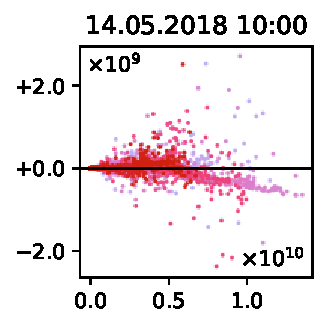
\includegraphics[width=0.30\textwidth,valign=t]{evaluation/figures/perturbations/perturbation-14.05.2018:10.00-anthropogenic-mul-1.01.pdf}
    \end{subfigure}
    \begin{subfigure}
        \centering
        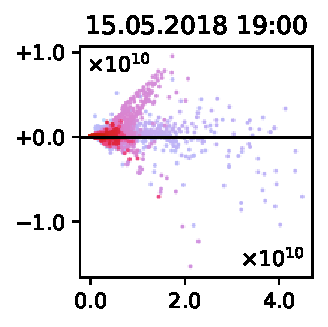
\includegraphics[width=0.30\textwidth,valign=t]{evaluation/figures/perturbations/perturbation-15.05.2018:19.00-anthropogenic-mul-1.01.pdf}
    \end{subfigure}
    \begin{subfigure}
        \centering
        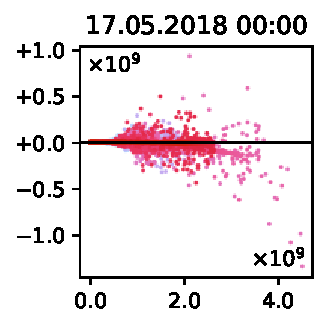
\includegraphics[width=0.30\textwidth,valign=t]{evaluation/figures/perturbations/perturbation-17.05.2018:00.00-anthropogenic-mul-1.01.pdf}
    \end{subfigure}

    \begin{subfigure}
        \centering
        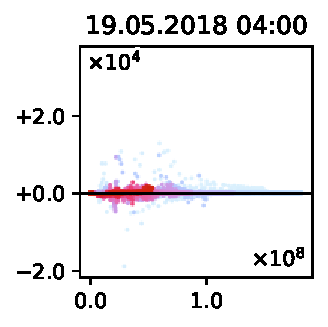
\includegraphics[width=0.30\textwidth,valign=t]{evaluation/figures/perturbations/perturbation-19.05.2018:04.00-anthropogenic-mul-1.01.pdf}
    \end{subfigure}
    \begin{subfigure}
        \centering
        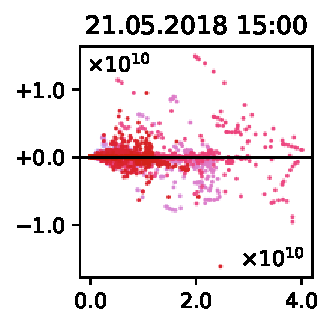
\includegraphics[width=0.30\textwidth,valign=t]{evaluation/figures/perturbations/perturbation-21.05.2018:15.00-anthropogenic-mul-1.01.pdf}
    \end{subfigure}
    \begin{subfigure}
        \centering
        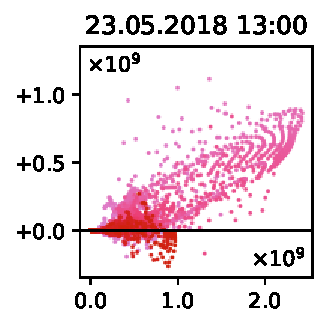
\includegraphics[width=0.30\textwidth,valign=t]{evaluation/figures/perturbations/perturbation-23.05.2018:13.00-anthropogenic-mul-1.01.pdf}
    \end{subfigure}

    \caption[Anthropogenic emissions$\times 1.01$ perturbation SOSAA results]{Anthropogenic emissions$\times 1.01$ perturbation results from the SOSAA model. The change in CCN is plotted on the y-axis against the baseline CCN concentration on the x-axis.}
    \label{fig:sosaa-perturbation-anthropogenic-mul-1.01}
\end{figure}

\begin{figure}[H]
    \centering
    \begin{subfigure}
        \centering
        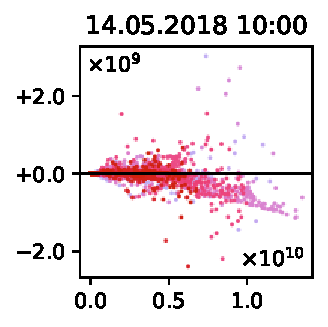
\includegraphics[width=0.30\textwidth,valign=t]{evaluation/figures/perturbations/perturbation-14.05.2018:10.00-anthropogenic-div-1.01.pdf}
    \end{subfigure}
    \begin{subfigure}
        \centering
        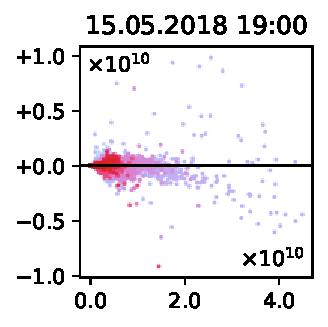
\includegraphics[width=0.30\textwidth,valign=t]{evaluation/figures/perturbations/perturbation-15.05.2018:19.00-anthropogenic-div-1.01.pdf}
    \end{subfigure}
    \begin{subfigure}
        \centering
        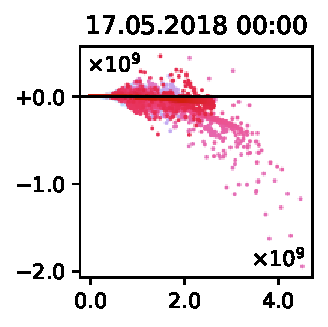
\includegraphics[width=0.30\textwidth,valign=t]{evaluation/figures/perturbations/perturbation-17.05.2018:00.00-anthropogenic-div-1.01.pdf}
    \end{subfigure}

    \begin{subfigure}
        \centering
        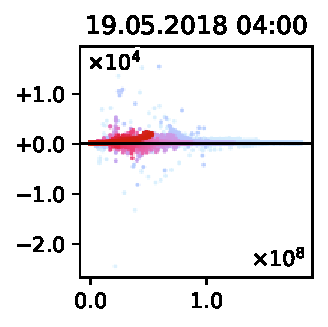
\includegraphics[width=0.30\textwidth,valign=t]{evaluation/figures/perturbations/perturbation-19.05.2018:04.00-anthropogenic-div-1.01.pdf}
    \end{subfigure}
    \begin{subfigure}
        \centering
        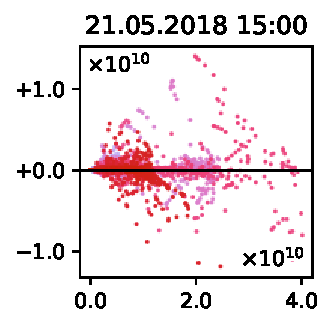
\includegraphics[width=0.30\textwidth,valign=t]{evaluation/figures/perturbations/perturbation-21.05.2018:15.00-anthropogenic-div-1.01.pdf}
    \end{subfigure}
    \begin{subfigure}
        \centering
        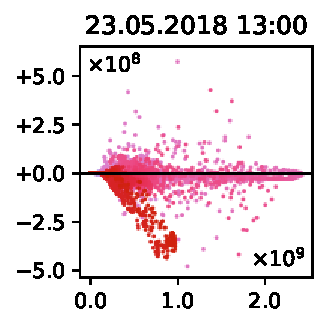
\includegraphics[width=0.30\textwidth,valign=t]{evaluation/figures/perturbations/perturbation-23.05.2018:13.00-anthropogenic-div-1.01.pdf}
    \end{subfigure}

    \caption[Anthropogenic emissions$\div 1.01$ perturbation SOSAA results]{Anthropogenic emissions$\div 1.01$ perturbation results from the SOSAA model. The change in CCN is plotted on the y-axis against the baseline CCN concentration on the x-axis.}
    \label{fig:sosaa-perturbation-anthropogenic-div-1.01}
\end{figure}

\begin{figure}[H]
    \centering
    \begin{subfigure}
        \centering
        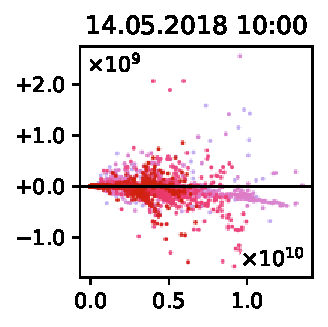
\includegraphics[width=0.30\textwidth,valign=t]{evaluation/figures/perturbations/perturbation-14.05.2018:10.00-temperature-add-0.04K.pdf}
    \end{subfigure}
    \begin{subfigure}
        \centering
        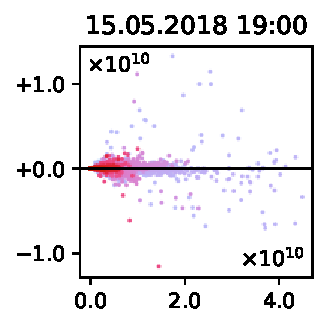
\includegraphics[width=0.30\textwidth,valign=t]{evaluation/figures/perturbations/perturbation-15.05.2018:19.00-temperature-add-0.04K.pdf}
    \end{subfigure}
    \begin{subfigure}
        \centering
        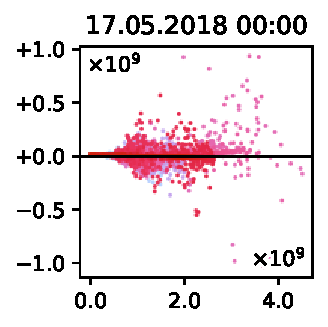
\includegraphics[width=0.30\textwidth,valign=t]{evaluation/figures/perturbations/perturbation-17.05.2018:00.00-temperature-add-0.04K.pdf}
    \end{subfigure}

    \begin{subfigure}
        \centering
        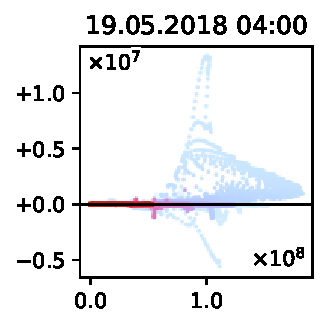
\includegraphics[width=0.30\textwidth,valign=t]{evaluation/figures/perturbations/perturbation-19.05.2018:04.00-temperature-add-0.04K.pdf}
    \end{subfigure}
    \begin{subfigure}
        \centering
        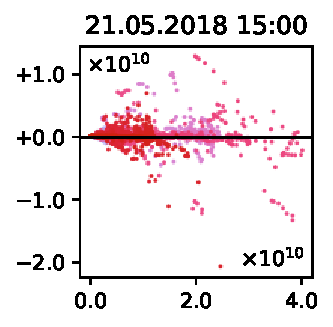
\includegraphics[width=0.30\textwidth,valign=t]{evaluation/figures/perturbations/perturbation-21.05.2018:15.00-temperature-add-0.04K.pdf}
    \end{subfigure}
    \begin{subfigure}
        \centering
        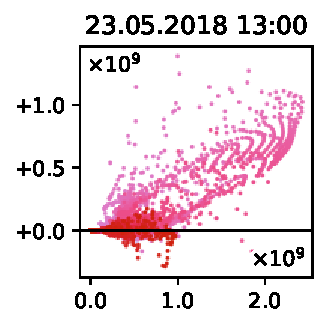
\includegraphics[width=0.30\textwidth,valign=t]{evaluation/figures/perturbations/perturbation-23.05.2018:13.00-temperature-add-0.04K.pdf}
    \end{subfigure}

    \caption[Temperature$+ 0.04\text{K}$ perturbation SOSAA results]{Air temperature$+ 0.04\text{K}$ perturbation results from the SOSAA model. The change in CCN is plotted on the y-axis against the baseline CCN concentration on the x-axis.}
    \label{fig:sosaa-perturbation-temperature-add-0.04K}
\end{figure}

\begin{figure}[H]
    \centering
    \begin{subfigure}
        \centering
        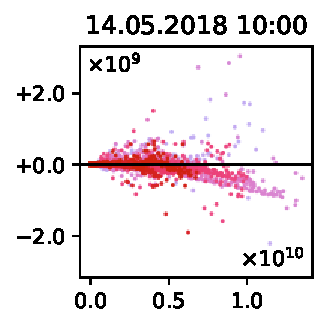
\includegraphics[width=0.30\textwidth,valign=t]{evaluation/figures/perturbations/perturbation-14.05.2018:10.00-temperature-sub-0.04K.pdf}
    \end{subfigure}
    \begin{subfigure}
        \centering
        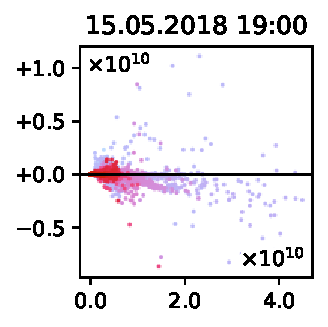
\includegraphics[width=0.30\textwidth,valign=t]{evaluation/figures/perturbations/perturbation-15.05.2018:19.00-temperature-sub-0.04K.pdf}
    \end{subfigure}
    \begin{subfigure}
        \centering
        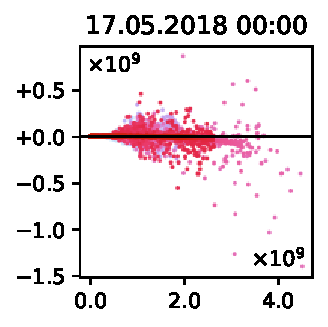
\includegraphics[width=0.30\textwidth,valign=t]{evaluation/figures/perturbations/perturbation-17.05.2018:00.00-temperature-sub-0.04K.pdf}
    \end{subfigure}

    \begin{subfigure}
        \centering
        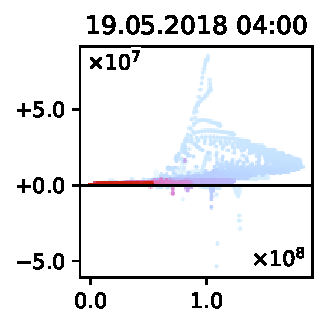
\includegraphics[width=0.30\textwidth,valign=t]{evaluation/figures/perturbations/perturbation-19.05.2018:04.00-temperature-sub-0.04K.pdf}
    \end{subfigure}
    \begin{subfigure}
        \centering
        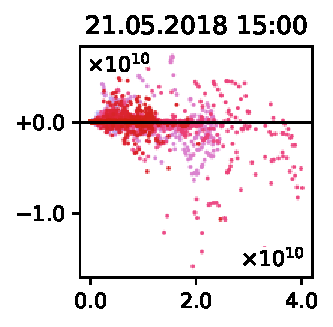
\includegraphics[width=0.30\textwidth,valign=t]{evaluation/figures/perturbations/perturbation-21.05.2018:15.00-temperature-sub-0.04K.pdf}
    \end{subfigure}
    \begin{subfigure}
        \centering
        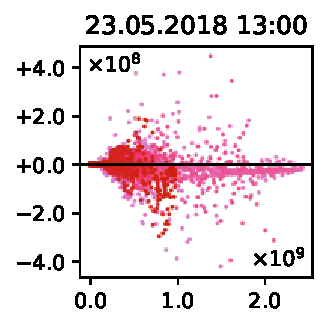
\includegraphics[width=0.30\textwidth,valign=t]{evaluation/figures/perturbations/perturbation-23.05.2018:13.00-temperature-sub-0.04K.pdf}
    \end{subfigure}

    \caption[Temperature$- 0.04\text{K}$ perturbation SOSAA results]{Air temperature$- 0.04\text{K}$ perturbation results from the SOSAA model. The change in CCN is plotted on the y-axis against the baseline CCN concentration on the x-axis.}
    \label{fig:sosaa-perturbation-temperature-sub-0.04K}
\end{figure}

\begin{figure}[H]
    \centering
    \begin{subfigure}
        \centering
        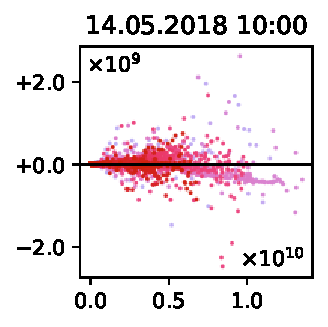
\includegraphics[width=0.30\textwidth,valign=t]{evaluation/figures/perturbations/perturbation-14.05.2018:10.00-aerosols-mul-1.01.pdf}
    \end{subfigure}
    \begin{subfigure}
        \centering
        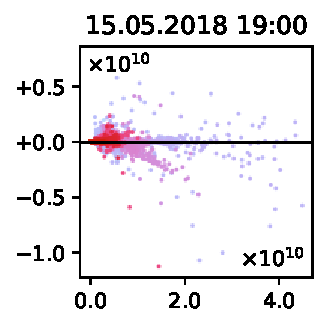
\includegraphics[width=0.30\textwidth,valign=t]{evaluation/figures/perturbations/perturbation-15.05.2018:19.00-aerosols-mul-1.01.pdf}
    \end{subfigure}
    \begin{subfigure}
        \centering
        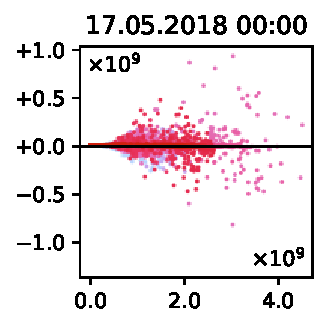
\includegraphics[width=0.30\textwidth,valign=t]{evaluation/figures/perturbations/perturbation-17.05.2018:00.00-aerosols-mul-1.01.pdf}
    \end{subfigure}

    \begin{subfigure}
        \centering
        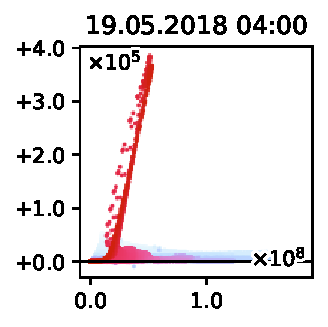
\includegraphics[width=0.30\textwidth,valign=t]{evaluation/figures/perturbations/perturbation-19.05.2018:04.00-aerosols-mul-1.01.pdf}
    \end{subfigure}
    \begin{subfigure}
        \centering
        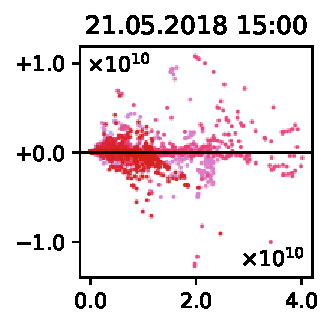
\includegraphics[width=0.30\textwidth,valign=t]{evaluation/figures/perturbations/perturbation-21.05.2018:15.00-aerosols-mul-1.01.pdf}
    \end{subfigure}
    \begin{subfigure}
        \centering
        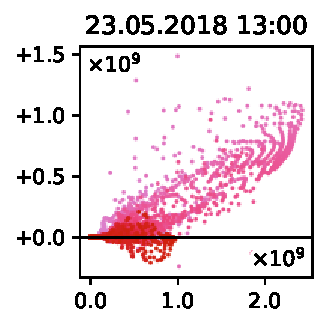
\includegraphics[width=0.30\textwidth,valign=t]{evaluation/figures/perturbations/perturbation-23.05.2018:13.00-aerosols-mul-1.01.pdf}
    \end{subfigure}

    \caption[Aerosol emissions$\times 1.01$ perturbation SOSAA results]{Aerosol emissions$\times 1.01$ perturbation results from the SOSAA model. The change in CCN is plotted on the y-axis against the baseline CCN concentration on the x-axis.}
    \label{fig:sosaa-perturbation-aerosols-mul-1.01}
\end{figure}

\begin{figure}[H]
    \centering
    \begin{subfigure}
        \centering
        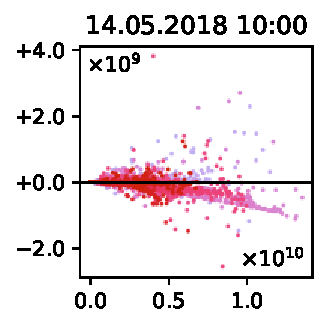
\includegraphics[width=0.30\textwidth,valign=t]{evaluation/figures/perturbations/perturbation-14.05.2018:10.00-aerosols-div-1.01.pdf}
    \end{subfigure}
    \begin{subfigure}
        \centering
        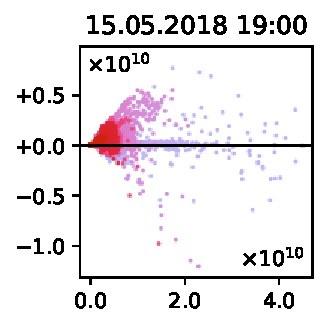
\includegraphics[width=0.30\textwidth,valign=t]{evaluation/figures/perturbations/perturbation-15.05.2018:19.00-aerosols-div-1.01.pdf}
    \end{subfigure}
    \begin{subfigure}
        \centering
        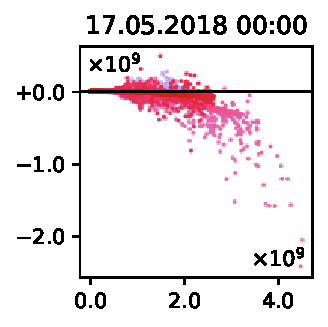
\includegraphics[width=0.30\textwidth,valign=t]{evaluation/figures/perturbations/perturbation-17.05.2018:00.00-aerosols-div-1.01.pdf}
    \end{subfigure}

    \begin{subfigure}
        \centering
        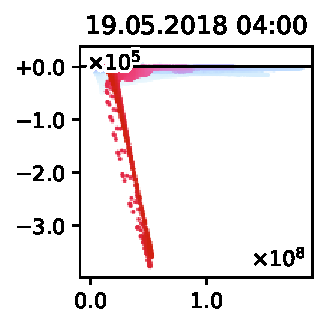
\includegraphics[width=0.30\textwidth,valign=t]{evaluation/figures/perturbations/perturbation-19.05.2018:04.00-aerosols-div-1.01.pdf}
    \end{subfigure}
    \begin{subfigure}
        \centering
        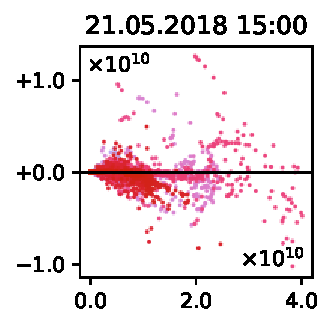
\includegraphics[width=0.30\textwidth,valign=t]{evaluation/figures/perturbations/perturbation-21.05.2018:15.00-aerosols-div-1.01.pdf}
    \end{subfigure}
    \begin{subfigure}
        \centering
        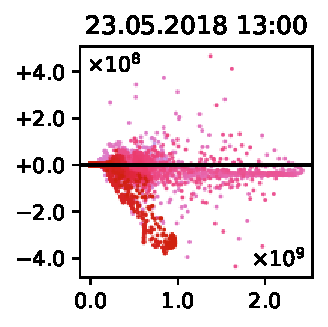
\includegraphics[width=0.30\textwidth,valign=t]{evaluation/figures/perturbations/perturbation-23.05.2018:13.00-aerosols-div-1.01.pdf}
    \end{subfigure}

    \caption[Aerosol emissions$\div 1.01$ perturbation SOSAA results]{Aerosol emissions$\div 1.01$ perturbation results from the SOSAA model. The change in CCN is plotted on the y-axis against the baseline CCN concentration on the x-axis.}
    \label{fig:sosaa-perturbation-aerosols-div-1.01}
\end{figure}

\begin{figure}[H]
    \centering
    \begin{subfigure}
        \centering
        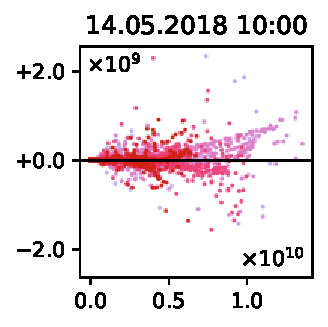
\includegraphics[width=0.30\textwidth,valign=t]{evaluation/figures/perturbations/perturbation-14.05.2018:10.00-biogenic-mul-1.01.pdf}
    \end{subfigure}
    \begin{subfigure}
        \centering
        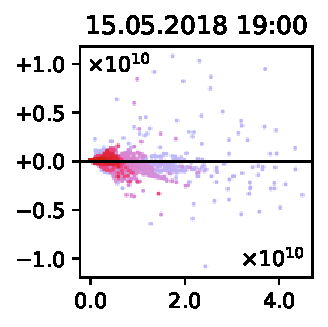
\includegraphics[width=0.30\textwidth,valign=t]{evaluation/figures/perturbations/perturbation-15.05.2018:19.00-biogenic-mul-1.01.pdf}
    \end{subfigure}
    \begin{subfigure}
        \centering
        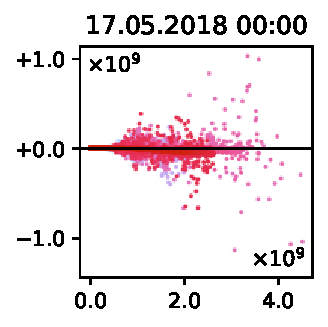
\includegraphics[width=0.30\textwidth,valign=t]{evaluation/figures/perturbations/perturbation-17.05.2018:00.00-biogenic-mul-1.01.pdf}
    \end{subfigure}

    \begin{subfigure}
        \centering
        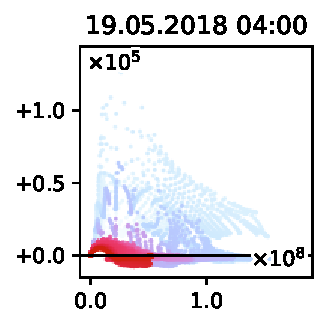
\includegraphics[width=0.30\textwidth,valign=t]{evaluation/figures/perturbations/perturbation-19.05.2018:04.00-biogenic-mul-1.01.pdf}
    \end{subfigure}
    \begin{subfigure}
        \centering
        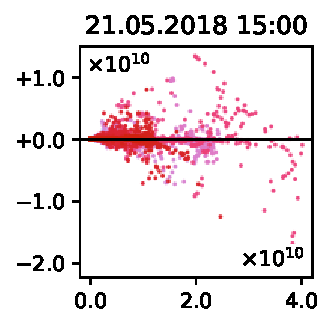
\includegraphics[width=0.30\textwidth,valign=t]{evaluation/figures/perturbations/perturbation-21.05.2018:15.00-biogenic-mul-1.01.pdf}
    \end{subfigure}
    \begin{subfigure}
        \centering
        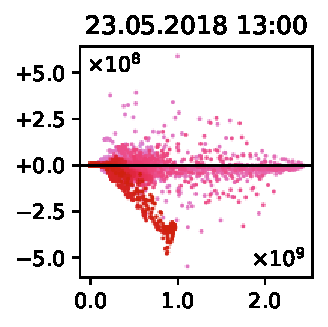
\includegraphics[width=0.30\textwidth,valign=t]{evaluation/figures/perturbations/perturbation-23.05.2018:13.00-biogenic-mul-1.01.pdf}
    \end{subfigure}

    \caption[Biogenic emissions$\times 1.01$ perturbation SOSAA results]{Biogenic (non-terpene) emissions$\times 1.01$ perturbation results from the SOSAA model. The change in CCN is plotted on the y-axis against the baseline CCN concentration on the x-axis.}
    \label{fig:sosaa-perturbation-biogenic-mul-1.01}
\end{figure}

\begin{figure}[H]
    \centering
    \begin{subfigure}
        \centering
        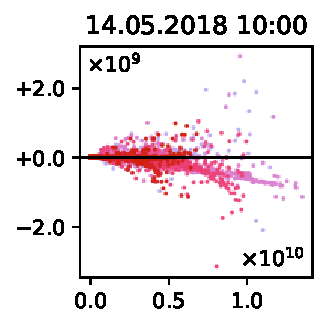
\includegraphics[width=0.30\textwidth,valign=t]{evaluation/figures/perturbations/perturbation-14.05.2018:10.00-biogenic-div-1.01.pdf}
    \end{subfigure}
    \begin{subfigure}
        \centering
        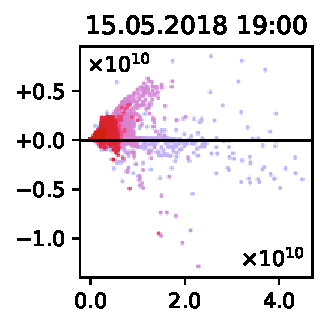
\includegraphics[width=0.30\textwidth,valign=t]{evaluation/figures/perturbations/perturbation-15.05.2018:19.00-biogenic-div-1.01.pdf}
    \end{subfigure}
    \begin{subfigure}
        \centering
        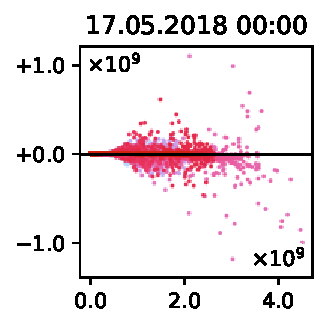
\includegraphics[width=0.30\textwidth,valign=t]{evaluation/figures/perturbations/perturbation-17.05.2018:00.00-biogenic-div-1.01.pdf}
    \end{subfigure}

    \begin{subfigure}
        \centering
        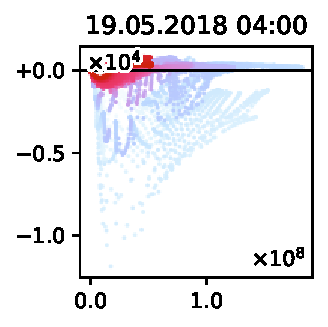
\includegraphics[width=0.30\textwidth,valign=t]{evaluation/figures/perturbations/perturbation-19.05.2018:04.00-biogenic-div-1.01.pdf}
    \end{subfigure}
    \begin{subfigure}
        \centering
        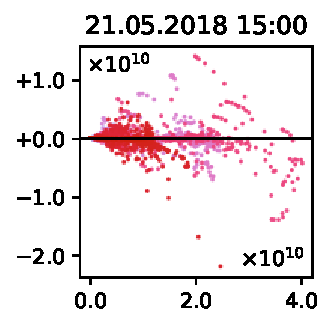
\includegraphics[width=0.30\textwidth,valign=t]{evaluation/figures/perturbations/perturbation-21.05.2018:15.00-biogenic-div-1.01.pdf}
    \end{subfigure}
    \begin{subfigure}
        \centering
        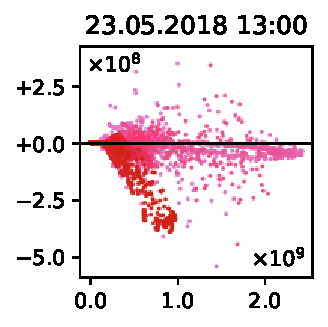
\includegraphics[width=0.30\textwidth,valign=t]{evaluation/figures/perturbations/perturbation-23.05.2018:13.00-biogenic-div-1.01.pdf}
    \end{subfigure}

    \caption[Biogenic emissions$\div 1.01$ perturbation SOSAA results]{Biogenic (non-terpene) emissions$\div 1.01$ perturbation results from the SOSAA model. The change in CCN is plotted on the y-axis against the baseline CCN concentration on the x-axis.}
    \label{fig:sosaa-perturbation-biogenic-div-1.01}
\end{figure}

\begin{figure}[H]
    \centering
    \begin{subfigure}
        \centering
        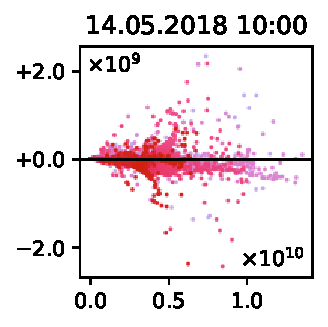
\includegraphics[width=0.30\textwidth,valign=t]{evaluation/figures/perturbations/perturbation-14.05.2018:10.00-nox-mul-1.01.pdf}
    \end{subfigure}
    \begin{subfigure}
        \centering
        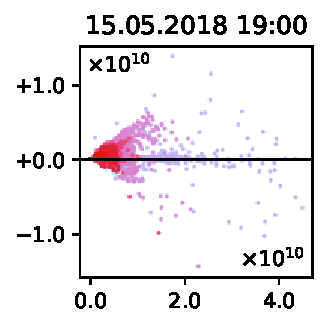
\includegraphics[width=0.30\textwidth,valign=t]{evaluation/figures/perturbations/perturbation-15.05.2018:19.00-nox-mul-1.01.pdf}
    \end{subfigure}
    \begin{subfigure}
        \centering
        \includegraphics[width=0.30\textwidth,valign=t]{evaluation/figures/perturbations/perturbation-17.05.2018:00.00-nox-mul-1.01.pdf}
    \end{subfigure}

    \begin{subfigure}
        \centering
        \includegraphics[width=0.30\textwidth,valign=t]{evaluation/figures/perturbations/perturbation-19.05.2018:04.00-nox-mul-1.01.pdf}
    \end{subfigure}
    \begin{subfigure}
        \centering
        \includegraphics[width=0.30\textwidth,valign=t]{evaluation/figures/perturbations/perturbation-21.05.2018:15.00-nox-mul-1.01.pdf}
    \end{subfigure}
    \begin{subfigure}
        \centering
        \includegraphics[width=0.30\textwidth,valign=t]{evaluation/figures/perturbations/perturbation-23.05.2018:13.00-nox-mul-1.01.pdf}
    \end{subfigure}

    \caption[$\text{NO}_x$ emissions$\times 1.01$ perturbation SOSAA results]{Anthropogenic $\text{NO}_x$ emissions$\times 1.01$ perturbation results from the SOSAA model. The change in CCN is plotted on the y-axis against the baseline CCN concentration on the x-axis.}
    \label{fig:sosaa-perturbation-nox-mul-1.01}
\end{figure}

\begin{figure}[H]
    \centering
    \begin{subfigure}
        \centering
        \includegraphics[width=0.30\textwidth,valign=t]{evaluation/figures/perturbations/perturbation-14.05.2018:10.00-nox-div-1.01.pdf}
    \end{subfigure}
    \begin{subfigure}
        \centering
        \includegraphics[width=0.30\textwidth,valign=t]{evaluation/figures/perturbations/perturbation-15.05.2018:19.00-nox-div-1.01.pdf}
    \end{subfigure}
    \begin{subfigure}
        \centering
        \includegraphics[width=0.30\textwidth,valign=t]{evaluation/figures/perturbations/perturbation-17.05.2018:00.00-nox-div-1.01.pdf}
    \end{subfigure}

    \begin{subfigure}
        \centering
        \includegraphics[width=0.30\textwidth,valign=t]{evaluation/figures/perturbations/perturbation-19.05.2018:04.00-nox-div-1.01.pdf}
    \end{subfigure}
    \begin{subfigure}
        \centering
        \includegraphics[width=0.30\textwidth,valign=t]{evaluation/figures/perturbations/perturbation-21.05.2018:15.00-nox-div-1.01.pdf}
    \end{subfigure}
    \begin{subfigure}
        \centering
        \includegraphics[width=0.30\textwidth,valign=t]{evaluation/figures/perturbations/perturbation-23.05.2018:13.00-nox-div-1.01.pdf}
    \end{subfigure}

    \caption[$\text{NO}_x$ emissions$\div 1.01$ perturbation SOSAA results]{Anthropogenic $\text{NO}_x$ emissions$\div 1.01$ perturbation results from the SOSAA model. The change in CCN is plotted on the y-axis against the baseline CCN concentration on the x-axis.}
    \label{fig:sosaa-perturbation-nox-div-1.01}
\end{figure}

\begin{figure}[H]
    \centering
    \begin{subfigure}
        \centering
        \includegraphics[width=0.30\textwidth,valign=t]{evaluation/figures/perturbations/perturbation-14.05.2018:10.00-so2-mul-1.01.pdf}
    \end{subfigure}
    \begin{subfigure}
        \centering
        \includegraphics[width=0.30\textwidth,valign=t]{evaluation/figures/perturbations/perturbation-15.05.2018:19.00-so2-mul-1.01.pdf}
    \end{subfigure}
    \begin{subfigure}
        \centering
        \includegraphics[width=0.30\textwidth,valign=t]{evaluation/figures/perturbations/perturbation-17.05.2018:00.00-so2-mul-1.01.pdf}
    \end{subfigure}

    \begin{subfigure}
        \centering
        \includegraphics[width=0.30\textwidth,valign=t]{evaluation/figures/perturbations/perturbation-19.05.2018:04.00-so2-mul-1.01.pdf}
    \end{subfigure}
    \begin{subfigure}
        \centering
        \includegraphics[width=0.30\textwidth,valign=t]{evaluation/figures/perturbations/perturbation-21.05.2018:15.00-so2-mul-1.01.pdf}
    \end{subfigure}
    \begin{subfigure}
        \centering
        \includegraphics[width=0.30\textwidth,valign=t]{evaluation/figures/perturbations/perturbation-23.05.2018:13.00-so2-mul-1.01.pdf}
    \end{subfigure}

    \caption[$\text{SO}_2$ emissions$\times 1.01$ perturbation SOSAA results]{Anthropogenic $\text{SO}_2$ emissions$\times 1.01$ perturbation results from the SOSAA model. The change in CCN is plotted on the y-axis against the baseline CCN concentration on the x-axis.}
    \label{fig:sosaa-perturbation-so2-mul-1.01}
\end{figure}

\begin{figure}[H]
    \centering
    \begin{subfigure}
        \centering
        \includegraphics[width=0.30\textwidth,valign=t]{evaluation/figures/perturbations/perturbation-14.05.2018:10.00-so2-div-1.01.pdf}
    \end{subfigure}
    \begin{subfigure}
        \centering
        \includegraphics[width=0.30\textwidth,valign=t]{evaluation/figures/perturbations/perturbation-15.05.2018:19.00-so2-div-1.01.pdf}
    \end{subfigure}
    \begin{subfigure}
        \centering
        \includegraphics[width=0.30\textwidth,valign=t]{evaluation/figures/perturbations/perturbation-17.05.2018:00.00-so2-div-1.01.pdf}
    \end{subfigure}

    \begin{subfigure}
        \centering
        \includegraphics[width=0.30\textwidth,valign=t]{evaluation/figures/perturbations/perturbation-19.05.2018:04.00-so2-div-1.01.pdf}
    \end{subfigure}
    \begin{subfigure}
        \centering
        \includegraphics[width=0.30\textwidth,valign=t]{evaluation/figures/perturbations/perturbation-21.05.2018:15.00-so2-div-1.01.pdf}
    \end{subfigure}
    \begin{subfigure}
        \centering
        \includegraphics[width=0.30\textwidth,valign=t]{evaluation/figures/perturbations/perturbation-23.05.2018:13.00-so2-div-1.01.pdf}
    \end{subfigure}

    \caption[$\text{SO}_2$ emissions$\div 1.01$ perturbation SOSAA results]{Anthropogenic $\text{SO}_2$ emissions$\div 1.01$ perturbation results from the SOSAA model. The change in CCN is plotted on the y-axis against the baseline CCN concentration on the x-axis.}
    \label{fig:sosaa-perturbation-so2-div-1.01}
\end{figure}

\begin{figure}[H]
    \centering
    \begin{subfigure}
        \centering
        \includegraphics[width=0.30\textwidth,valign=t]{evaluation/figures/perturbations/perturbation-14.05.2018:10.00-monoterpenes-mul-1.01.pdf}
    \end{subfigure}
    \begin{subfigure}
        \centering
        \includegraphics[width=0.30\textwidth,valign=t]{evaluation/figures/perturbations/perturbation-15.05.2018:19.00-monoterpenes-mul-1.01.pdf}
    \end{subfigure}
    \begin{subfigure}
        \centering
        \includegraphics[width=0.30\textwidth,valign=t]{evaluation/figures/perturbations/perturbation-17.05.2018:00.00-monoterpenes-mul-1.01.pdf}
    \end{subfigure}

    \begin{subfigure}
        \centering
        \includegraphics[width=0.30\textwidth,valign=t]{evaluation/figures/perturbations/perturbation-19.05.2018:04.00-monoterpenes-mul-1.01.pdf}
    \end{subfigure}
    \begin{subfigure}
        \centering
        \includegraphics[width=0.30\textwidth,valign=t]{evaluation/figures/perturbations/perturbation-21.05.2018:15.00-monoterpenes-mul-1.01.pdf}
    \end{subfigure}
    \begin{subfigure}
        \centering
        \includegraphics[width=0.30\textwidth,valign=t]{evaluation/figures/perturbations/perturbation-23.05.2018:13.00-monoterpenes-mul-1.01.pdf}
    \end{subfigure}

    \caption[Monoterpene emissions$\times 1.01$ perturbation SOSAA results]{Monoterpene emissions$\times 1.01$ perturbation results from the SOSAA model. The change in CCN is plotted on the y-axis against the baseline CCN concentration on the x-axis.}
    \label{fig:sosaa-perturbation-monoterpenes-mul-1.01}
\end{figure}

\begin{figure}[H]
    \centering
    \begin{subfigure}
        \centering
        \includegraphics[width=0.30\textwidth,valign=t]{evaluation/figures/perturbations/perturbation-14.05.2018:10.00-monoterpenes-div-1.01.pdf}
    \end{subfigure}
    \begin{subfigure}
        \centering
        \includegraphics[width=0.30\textwidth,valign=t]{evaluation/figures/perturbations/perturbation-15.05.2018:19.00-monoterpenes-div-1.01.pdf}
    \end{subfigure}
    \begin{subfigure}
        \centering
        \includegraphics[width=0.30\textwidth,valign=t]{evaluation/figures/perturbations/perturbation-17.05.2018:00.00-monoterpenes-div-1.01.pdf}
    \end{subfigure}

    \begin{subfigure}
        \centering
        \includegraphics[width=0.30\textwidth,valign=t]{evaluation/figures/perturbations/perturbation-19.05.2018:04.00-monoterpenes-div-1.01.pdf}
    \end{subfigure}
    \begin{subfigure}
        \centering
        \includegraphics[width=0.30\textwidth,valign=t]{evaluation/figures/perturbations/perturbation-21.05.2018:15.00-monoterpenes-div-1.01.pdf}
    \end{subfigure}
    \begin{subfigure}
        \centering
        \includegraphics[width=0.30\textwidth,valign=t]{evaluation/figures/perturbations/perturbation-23.05.2018:13.00-monoterpenes-div-1.01.pdf}
    \end{subfigure}

    \caption[Monoterpene emissions$\div 1.01$ perturbation SOSAA results]{Monoterpene emissions$\div 1.01$ perturbation results from the SOSAA model. The change in CCN is plotted on the y-axis against the baseline CCN concentration on the x-axis.}
    \label{fig:sosaa-perturbation-monoterpenes-div-1.01}
\end{figure}

\begin{figure}[H]
    \centering
    \begin{subfigure}
        \centering
        \includegraphics[width=0.30\textwidth,valign=t]{evaluation/figures/perturbations/perturbation-14.05.2018:10.00-sesquiterpenes-mul-1.01.pdf}
    \end{subfigure}
    \begin{subfigure}
        \centering
        \includegraphics[width=0.30\textwidth,valign=t]{evaluation/figures/perturbations/perturbation-15.05.2018:19.00-sesquiterpenes-mul-1.01.pdf}
    \end{subfigure}
    \begin{subfigure}
        \centering
        \includegraphics[width=0.30\textwidth,valign=t]{evaluation/figures/perturbations/perturbation-17.05.2018:00.00-sesquiterpenes-mul-1.01.pdf}
    \end{subfigure}

    \begin{subfigure}
        \centering
        \includegraphics[width=0.30\textwidth,valign=t]{evaluation/figures/perturbations/perturbation-19.05.2018:04.00-sesquiterpenes-mul-1.01.pdf}
    \end{subfigure}
    \begin{subfigure}
        \centering
        \includegraphics[width=0.30\textwidth,valign=t]{evaluation/figures/perturbations/perturbation-21.05.2018:15.00-sesquiterpenes-mul-1.01.pdf}
    \end{subfigure}
    \begin{subfigure}
        \centering
        \includegraphics[width=0.30\textwidth,valign=t]{evaluation/figures/perturbations/perturbation-23.05.2018:13.00-sesquiterpenes-mul-1.01.pdf}
    \end{subfigure}
    
    \caption[Sesquiterpene emissions$\times 1.01$ perturbation SOSAA results]{Sesquiterpene emissions$\times 1.01$ perturbation results from the SOSAA model. The change in CCN is plotted on the y-axis against the baseline CCN concentration on the x-axis.}
    \label{fig:sosaa-perturbation-sesquiterpenes-mul-1.01}
\end{figure}

\begin{figure}[H]
    \centering
    \begin{subfigure}
        \centering
        \includegraphics[width=0.30\textwidth,valign=t]{evaluation/figures/perturbations/perturbation-14.05.2018:10.00-sesquiterpenes-div-1.01.pdf}
    \end{subfigure}
    \begin{subfigure}
        \centering
        \includegraphics[width=0.30\textwidth,valign=t]{evaluation/figures/perturbations/perturbation-15.05.2018:19.00-sesquiterpenes-div-1.01.pdf}
    \end{subfigure}
    \begin{subfigure}
        \centering
        \includegraphics[width=0.30\textwidth,valign=t]{evaluation/figures/perturbations/perturbation-17.05.2018:00.00-sesquiterpenes-div-1.01.pdf}
    \end{subfigure}

    \begin{subfigure}
        \centering
        \includegraphics[width=0.30\textwidth,valign=t]{evaluation/figures/perturbations/perturbation-19.05.2018:04.00-sesquiterpenes-div-1.01.pdf}
    \end{subfigure}
    \begin{subfigure}
        \centering
        \includegraphics[width=0.30\textwidth,valign=t]{evaluation/figures/perturbations/perturbation-21.05.2018:15.00-sesquiterpenes-div-1.01.pdf}
    \end{subfigure}
    \begin{subfigure}
        \centering
        \includegraphics[width=0.30\textwidth,valign=t]{evaluation/figures/perturbations/perturbation-23.05.2018:13.00-sesquiterpenes-div-1.01.pdf}
    \end{subfigure}
    
    \caption[Sesquiterpene emissions$\div 1.01$ perturbation SOSAA results]{Sesquiterpene emissions$\div 1.01$ perturbation results from the SOSAA model. The change in CCN is plotted on the y-axis against the baseline CCN concentration on the x-axis.}
    \label{fig:sosaa-perturbation-sesquiterpenes-div-1.01}
\end{figure}

\begin{figure}[H]
    \centering
    \begin{subfigure}
        \centering
        \includegraphics[width=0.30\textwidth,valign=t]{evaluation/figures/perturbations/perturbation-14.05.2018:10.00-anthropogenic-mul-1.5.pdf}
    \end{subfigure}
    \begin{subfigure}
        \centering
        \includegraphics[width=0.30\textwidth,valign=t]{evaluation/figures/perturbations/perturbation-15.05.2018:19.00-anthropogenic-mul-1.5.pdf}
    \end{subfigure}
    \begin{subfigure}
        \centering
        \includegraphics[width=0.30\textwidth,valign=t]{evaluation/figures/perturbations/perturbation-17.05.2018:00.00-anthropogenic-mul-1.5.pdf}
    \end{subfigure}

    \begin{subfigure}
        \centering
        \includegraphics[width=0.30\textwidth,valign=t]{evaluation/figures/perturbations/perturbation-19.05.2018:04.00-anthropogenic-mul-1.5.pdf}
    \end{subfigure}
    \begin{subfigure}
        \centering
        \includegraphics[width=0.30\textwidth,valign=t]{evaluation/figures/perturbations/perturbation-21.05.2018:15.00-anthropogenic-mul-1.5.pdf}
    \end{subfigure}
    \begin{subfigure}
        \centering
        \includegraphics[width=0.30\textwidth,valign=t]{evaluation/figures/perturbations/perturbation-23.05.2018:13.00-anthropogenic-mul-1.5.pdf}
    \end{subfigure}

    \caption[Anthropogenic emissions$\times 1.5$ perturbation SOSAA results]{Anthropogenic emissions$\times 1.5$ perturbation results from the SOSAA model. The change in CCN is plotted on the y-axis against the baseline CCN concentration on the x-axis.}
    \label{fig:sosaa-perturbation-anthropogenic-mul-1.5}
\end{figure}

\begin{figure}[H]
    \centering
    \begin{subfigure}
        \centering
        \includegraphics[width=0.30\textwidth,valign=t]{evaluation/figures/perturbations/perturbation-14.05.2018:10.00-anthropogenic-div-1.5.pdf}
    \end{subfigure}
    \begin{subfigure}
        \centering
        \includegraphics[width=0.30\textwidth,valign=t]{evaluation/figures/perturbations/perturbation-15.05.2018:19.00-anthropogenic-div-1.5.pdf}
    \end{subfigure}
    \begin{subfigure}
        \centering
        \includegraphics[width=0.30\textwidth,valign=t]{evaluation/figures/perturbations/perturbation-17.05.2018:00.00-anthropogenic-div-1.5.pdf}
    \end{subfigure}

    \begin{subfigure}
        \centering
        \includegraphics[width=0.30\textwidth,valign=t]{evaluation/figures/perturbations/perturbation-19.05.2018:04.00-anthropogenic-div-1.5.pdf}
    \end{subfigure}
    \begin{subfigure}
        \centering
        \includegraphics[width=0.30\textwidth,valign=t]{evaluation/figures/perturbations/perturbation-21.05.2018:15.00-anthropogenic-div-1.5.pdf}
    \end{subfigure}
    \begin{subfigure}
        \centering
        \includegraphics[width=0.30\textwidth,valign=t]{evaluation/figures/perturbations/perturbation-23.05.2018:13.00-anthropogenic-div-1.5.pdf}
    \end{subfigure}

    \caption[Anthropogenic emissions$\div 1.5$ perturbation SOSAA results]{Anthropogenic emissions$\div 1.5$ perturbation results from the SOSAA model. The change in CCN is plotted on the y-axis against the baseline CCN concentration on the x-axis.}
    \label{fig:sosaa-perturbation-anthropogenic-div-1.5}
\end{figure}

\begin{figure}[H]
    \centering
    \begin{subfigure}
        \centering
        \includegraphics[width=0.30\textwidth,valign=t]{evaluation/figures/perturbations/perturbation-14.05.2018:10.00-temperature-add-2K.pdf}
    \end{subfigure}
    \begin{subfigure}
        \centering
        \includegraphics[width=0.30\textwidth,valign=t]{evaluation/figures/perturbations/perturbation-15.05.2018:19.00-temperature-add-2K.pdf}
    \end{subfigure}
    \begin{subfigure}
        \centering
        \includegraphics[width=0.30\textwidth,valign=t]{evaluation/figures/perturbations/perturbation-17.05.2018:00.00-temperature-add-2K.pdf}
    \end{subfigure}

    \begin{subfigure}
        \centering
        \includegraphics[width=0.30\textwidth,valign=t]{evaluation/figures/perturbations/perturbation-19.05.2018:04.00-temperature-add-2K.pdf}
    \end{subfigure}
    \begin{subfigure}
        \centering
        \includegraphics[width=0.30\textwidth,valign=t]{evaluation/figures/perturbations/perturbation-21.05.2018:15.00-temperature-add-2K.pdf}
    \end{subfigure}
    \begin{subfigure}
        \centering
        \includegraphics[width=0.30\textwidth,valign=t]{evaluation/figures/perturbations/perturbation-23.05.2018:13.00-temperature-add-2K.pdf}
    \end{subfigure}

    \caption[Temperature$+ 2\text{K}$ perturbation SOSAA results]{Air temperature$+ 2\text{K}$ perturbation results from the SOSAA model. The change in CCN is plotted on the y-axis against the baseline CCN concentration on the x-axis.}
    \label{fig:sosaa-perturbation-temperature-add-2K}
\end{figure}

\begin{figure}[H]
    \centering
    \begin{subfigure}
        \centering
        \includegraphics[width=0.30\textwidth,valign=t]{evaluation/figures/perturbations/perturbation-14.05.2018:10.00-temperature-sub-2K.pdf}
    \end{subfigure}
    \begin{subfigure}
        \centering
        \includegraphics[width=0.30\textwidth,valign=t]{evaluation/figures/perturbations/perturbation-15.05.2018:19.00-temperature-sub-2K.pdf}
    \end{subfigure}
    \begin{subfigure}
        \centering
        \includegraphics[width=0.30\textwidth,valign=t]{evaluation/figures/perturbations/perturbation-17.05.2018:00.00-temperature-sub-2K.pdf}
    \end{subfigure}

    \begin{subfigure}
        \centering
        \includegraphics[width=0.30\textwidth,valign=t]{evaluation/figures/perturbations/perturbation-19.05.2018:04.00-temperature-sub-2K.pdf}
    \end{subfigure}
    \begin{subfigure}
        \centering
        \includegraphics[width=0.30\textwidth,valign=t]{evaluation/figures/perturbations/perturbation-21.05.2018:15.00-temperature-sub-2K.pdf}
    \end{subfigure}
    \begin{subfigure}
        \centering
        \includegraphics[width=0.30\textwidth,valign=t]{evaluation/figures/perturbations/perturbation-23.05.2018:13.00-temperature-sub-2K.pdf}
    \end{subfigure}

    \caption[Temperature$- 2\text{K}$ perturbation SOSAA results]{Air temperature$- 2\text{K}$ perturbation results from the SOSAA model. The change in CCN is plotted on the y-axis against the baseline CCN concentration on the x-axis.}
    \label{fig:sosaa-perturbation-temperature-sub-2K}
\end{figure}

\begin{figure}[H]
    \centering
    \begin{subfigure}
        \centering
        \includegraphics[width=0.30\textwidth,valign=t]{evaluation/figures/perturbations/perturbation-14.05.2018:10.00-aerosols-mul-1.5.pdf}
    \end{subfigure}
    \begin{subfigure}
        \centering
        \includegraphics[width=0.30\textwidth,valign=t]{evaluation/figures/perturbations/perturbation-15.05.2018:19.00-aerosols-mul-1.5.pdf}
    \end{subfigure}
    \begin{subfigure}
        \centering
        \includegraphics[width=0.30\textwidth,valign=t]{evaluation/figures/perturbations/perturbation-17.05.2018:00.00-aerosols-mul-1.5.pdf}
    \end{subfigure}

    \begin{subfigure}
        \centering
        \includegraphics[width=0.30\textwidth,valign=t]{evaluation/figures/perturbations/perturbation-19.05.2018:04.00-aerosols-mul-1.5.pdf}
    \end{subfigure}
    \begin{subfigure}
        \centering
        \includegraphics[width=0.30\textwidth,valign=t]{evaluation/figures/perturbations/perturbation-21.05.2018:15.00-aerosols-mul-1.5.pdf}
    \end{subfigure}
    \begin{subfigure}
        \centering
        \includegraphics[width=0.30\textwidth,valign=t]{evaluation/figures/perturbations/perturbation-23.05.2018:13.00-aerosols-mul-1.5.pdf}
    \end{subfigure}

    \caption[Aerosol emissions$\times 1.5$ perturbation SOSAA results]{Aerosol emissions$\times 1.5$ perturbation results from the SOSAA model. The change in CCN is plotted on the y-axis against the baseline CCN concentration on the x-axis.}
    \label{fig:sosaa-perturbation-aerosols-mul-1.5}
\end{figure}

\begin{figure}[H]
    \centering
    \begin{subfigure}
        \centering
        \includegraphics[width=0.30\textwidth,valign=t]{evaluation/figures/perturbations/perturbation-14.05.2018:10.00-aerosols-div-1.5.pdf}
    \end{subfigure}
    \begin{subfigure}
        \centering
        \includegraphics[width=0.30\textwidth,valign=t]{evaluation/figures/perturbations/perturbation-15.05.2018:19.00-aerosols-div-1.5.pdf}
    \end{subfigure}
    \begin{subfigure}
        \centering
        \includegraphics[width=0.30\textwidth,valign=t]{evaluation/figures/perturbations/perturbation-17.05.2018:00.00-aerosols-div-1.5.pdf}
    \end{subfigure}

    \begin{subfigure}
        \centering
        \includegraphics[width=0.30\textwidth,valign=t]{evaluation/figures/perturbations/perturbation-19.05.2018:04.00-aerosols-div-1.5.pdf}
    \end{subfigure}
    \begin{subfigure}
        \centering
        \includegraphics[width=0.30\textwidth,valign=t]{evaluation/figures/perturbations/perturbation-21.05.2018:15.00-aerosols-div-1.5.pdf}
    \end{subfigure}
    \begin{subfigure}
        \centering
        \includegraphics[width=0.30\textwidth,valign=t]{evaluation/figures/perturbations/perturbation-23.05.2018:13.00-aerosols-div-1.5.pdf}
    \end{subfigure}

    \caption[Aerosol emissions$\div 1.5$ perturbation SOSAA results]{Aerosol emissions$\div 1.5$ perturbation results from the SOSAA model. The change in CCN is plotted on the y-axis against the baseline CCN concentration on the x-axis.}
    \label{fig:sosaa-perturbation-aerosols-div-1.5}
\end{figure}

\begin{figure}[H]
    \centering
    \begin{subfigure}
        \centering
        \includegraphics[width=0.30\textwidth,valign=t]{evaluation/figures/perturbations/perturbation-14.05.2018:10.00-biogenic-mul-1.5.pdf}
    \end{subfigure}
    \begin{subfigure}
        \centering
        \includegraphics[width=0.30\textwidth,valign=t]{evaluation/figures/perturbations/perturbation-15.05.2018:19.00-biogenic-mul-1.5.pdf}
    \end{subfigure}
    \begin{subfigure}
        \centering
        \includegraphics[width=0.30\textwidth,valign=t]{evaluation/figures/perturbations/perturbation-17.05.2018:00.00-biogenic-mul-1.5.pdf}
    \end{subfigure}

    \begin{subfigure}
        \centering
        \includegraphics[width=0.30\textwidth,valign=t]{evaluation/figures/perturbations/perturbation-19.05.2018:04.00-biogenic-mul-1.5.pdf}
    \end{subfigure}
    \begin{subfigure}
        \centering
        \includegraphics[width=0.30\textwidth,valign=t]{evaluation/figures/perturbations/perturbation-21.05.2018:15.00-biogenic-mul-1.5.pdf}
    \end{subfigure}
    \begin{subfigure}
        \centering
        \includegraphics[width=0.30\textwidth,valign=t]{evaluation/figures/perturbations/perturbation-23.05.2018:13.00-biogenic-mul-1.5.pdf}
    \end{subfigure}

    \caption[Biogenic emissions$\times 1.5$ perturbation SOSAA results]{Biogenic (non-terpene) emissions$\times 1.5$ perturbation results from the SOSAA model. The change in CCN is plotted on the y-axis against the baseline CCN concentration on the x-axis.}
    \label{fig:sosaa-perturbation-biogenic-mul-1.5}
\end{figure}

\begin{figure}[H]
    \centering
    \begin{subfigure}
        \centering
        \includegraphics[width=0.30\textwidth,valign=t]{evaluation/figures/perturbations/perturbation-14.05.2018:10.00-biogenic-div-1.5.pdf}
    \end{subfigure}
    \begin{subfigure}
        \centering
        \includegraphics[width=0.30\textwidth,valign=t]{evaluation/figures/perturbations/perturbation-15.05.2018:19.00-biogenic-div-1.5.pdf}
    \end{subfigure}
    \begin{subfigure}
        \centering
        \includegraphics[width=0.30\textwidth,valign=t]{evaluation/figures/perturbations/perturbation-17.05.2018:00.00-biogenic-div-1.5.pdf}
    \end{subfigure}

    \begin{subfigure}
        \centering
        \includegraphics[width=0.30\textwidth,valign=t]{evaluation/figures/perturbations/perturbation-19.05.2018:04.00-biogenic-div-1.5.pdf}
    \end{subfigure}
    \begin{subfigure}
        \centering
        \includegraphics[width=0.30\textwidth,valign=t]{evaluation/figures/perturbations/perturbation-21.05.2018:15.00-biogenic-div-1.5.pdf}
    \end{subfigure}
    \begin{subfigure}
        \centering
        \includegraphics[width=0.30\textwidth,valign=t]{evaluation/figures/perturbations/perturbation-23.05.2018:13.00-biogenic-div-1.5.pdf}
    \end{subfigure}

    \caption[Biogenic emissions$\div 1.5$ perturbation SOSAA results]{Biogenic (non-terpene) emissions$\div 1.5$ perturbation results from the SOSAA model. The change in CCN is plotted on the y-axis against the baseline CCN concentration on the x-axis.}
    \label{fig:sosaa-perturbation-biogenic-div-1.5}
\end{figure}

\begin{figure}[H]
    \centering
    \begin{subfigure}
        \centering
        \includegraphics[width=0.30\textwidth,valign=t]{evaluation/figures/perturbations/perturbation-14.05.2018:10.00-nox-mul-1.5.pdf}
    \end{subfigure}
    \begin{subfigure}
        \centering
        \includegraphics[width=0.30\textwidth,valign=t]{evaluation/figures/perturbations/perturbation-15.05.2018:19.00-nox-mul-1.5.pdf}
    \end{subfigure}
    \begin{subfigure}
        \centering
        \includegraphics[width=0.30\textwidth,valign=t]{evaluation/figures/perturbations/perturbation-17.05.2018:00.00-nox-mul-1.5.pdf}
    \end{subfigure}

    \begin{subfigure}
        \centering
        \includegraphics[width=0.30\textwidth,valign=t]{evaluation/figures/perturbations/perturbation-19.05.2018:04.00-nox-mul-1.5.pdf}
    \end{subfigure}
    \begin{subfigure}
        \centering
        \includegraphics[width=0.30\textwidth,valign=t]{evaluation/figures/perturbations/perturbation-21.05.2018:15.00-nox-mul-1.5.pdf}
    \end{subfigure}
    \begin{subfigure}
        \centering
        \includegraphics[width=0.30\textwidth,valign=t]{evaluation/figures/perturbations/perturbation-23.05.2018:13.00-nox-mul-1.5.pdf}
    \end{subfigure}

    \caption[$\text{NO}_x$ emissions$\times 1.5$ perturbation SOSAA results]{Anthropogenic $\text{NO}_x$ emissions$\times 1.5$ perturbation results from the SOSAA model. The change in CCN is plotted on the y-axis against the baseline CCN concentration on the x-axis.}
    \label{fig:sosaa-perturbation-nox-mul-1.5}
\end{figure}

\begin{figure}[H]
    \centering
    \begin{subfigure}
        \centering
        \includegraphics[width=0.30\textwidth,valign=t]{evaluation/figures/perturbations/perturbation-14.05.2018:10.00-nox-div-1.5.pdf}
    \end{subfigure}
    \begin{subfigure}
        \centering
        \includegraphics[width=0.30\textwidth,valign=t]{evaluation/figures/perturbations/perturbation-15.05.2018:19.00-nox-div-1.5.pdf}
    \end{subfigure}
    \begin{subfigure}
        \centering
        \includegraphics[width=0.30\textwidth,valign=t]{evaluation/figures/perturbations/perturbation-17.05.2018:00.00-nox-div-1.5.pdf}
    \end{subfigure}

    \begin{subfigure}
        \centering
        \includegraphics[width=0.30\textwidth,valign=t]{evaluation/figures/perturbations/perturbation-19.05.2018:04.00-nox-div-1.5.pdf}
    \end{subfigure}
    \begin{subfigure}
        \centering
        \includegraphics[width=0.30\textwidth,valign=t]{evaluation/figures/perturbations/perturbation-21.05.2018:15.00-nox-div-1.5.pdf}
    \end{subfigure}
    \begin{subfigure}
        \centering
        \includegraphics[width=0.30\textwidth,valign=t]{evaluation/figures/perturbations/perturbation-23.05.2018:13.00-nox-div-1.5.pdf}
    \end{subfigure}

    \caption[$\text{NO}_x$ emissions$\div 1.5$ perturbation SOSAA results]{Anthropogenic $\text{NO}_x$ emissions$\div 1.5$ perturbation results from the SOSAA model. The change in CCN is plotted on the y-axis against the baseline CCN concentration on the x-axis.}
    \label{fig:sosaa-perturbation-nox-div-1.5}
\end{figure}

\begin{figure}[H]
    \centering
    \begin{subfigure}
        \centering
        \includegraphics[width=0.30\textwidth,valign=t]{evaluation/figures/perturbations/perturbation-14.05.2018:10.00-so2-mul-1.5.pdf}
    \end{subfigure}
    \begin{subfigure}
        \centering
        \includegraphics[width=0.30\textwidth,valign=t]{evaluation/figures/perturbations/perturbation-15.05.2018:19.00-so2-mul-1.5.pdf}
    \end{subfigure}
    \begin{subfigure}
        \centering
        \includegraphics[width=0.30\textwidth,valign=t]{evaluation/figures/perturbations/perturbation-17.05.2018:00.00-so2-mul-1.5.pdf}
    \end{subfigure}

    \begin{subfigure}
        \centering
        \includegraphics[width=0.30\textwidth,valign=t]{evaluation/figures/perturbations/perturbation-19.05.2018:04.00-so2-mul-1.5.pdf}
    \end{subfigure}
    \begin{subfigure}
        \centering
        \includegraphics[width=0.30\textwidth,valign=t]{evaluation/figures/perturbations/perturbation-21.05.2018:15.00-so2-mul-1.5.pdf}
    \end{subfigure}
    \begin{subfigure}
        \centering
        \includegraphics[width=0.30\textwidth,valign=t]{evaluation/figures/perturbations/perturbation-23.05.2018:13.00-so2-mul-1.5.pdf}
    \end{subfigure}

    \caption[$\text{SO}_2$ emissions$\times 1.5$ perturbation SOSAA results]{Anthropogenic $\text{SO}_2$ emissions$\times 1.5$ perturbation results from the SOSAA model. The change in CCN is plotted on the y-axis against the baseline CCN concentration on the x-axis.}
    \label{fig:sosaa-perturbation-so2-mul-1.5}
\end{figure}

\begin{figure}[H]
    \centering
    \begin{subfigure}
        \centering
        \includegraphics[width=0.30\textwidth,valign=t]{evaluation/figures/perturbations/perturbation-14.05.2018:10.00-so2-div-1.5.pdf}
    \end{subfigure}
    \begin{subfigure}
        \centering
        \includegraphics[width=0.30\textwidth,valign=t]{evaluation/figures/perturbations/perturbation-15.05.2018:19.00-so2-div-1.5.pdf}
    \end{subfigure}
    \begin{subfigure}
        \centering
        \includegraphics[width=0.30\textwidth,valign=t]{evaluation/figures/perturbations/perturbation-17.05.2018:00.00-so2-div-1.5.pdf}
    \end{subfigure}

    \begin{subfigure}
        \centering
        \includegraphics[width=0.30\textwidth,valign=t]{evaluation/figures/perturbations/perturbation-19.05.2018:04.00-so2-div-1.5.pdf}
    \end{subfigure}
    \begin{subfigure}
        \centering
        \includegraphics[width=0.30\textwidth,valign=t]{evaluation/figures/perturbations/perturbation-21.05.2018:15.00-so2-div-1.5.pdf}
    \end{subfigure}
    \begin{subfigure}
        \centering
        \includegraphics[width=0.30\textwidth,valign=t]{evaluation/figures/perturbations/perturbation-23.05.2018:13.00-so2-div-1.5.pdf}
    \end{subfigure}

    \caption[$\text{SO}_2$ emissions$\div 1.5$ perturbation SOSAA results]{Anthropogenic $\text{SO}_2$ emissions$\div 1.5$ perturbation results from the SOSAA model. The change in CCN is plotted on the y-axis against the baseline CCN concentration on the x-axis.}
    \label{fig:sosaa-perturbation-so2-div-1.5}
\end{figure}

\begin{figure}[H]
    \centering
    \begin{subfigure}
        \centering
        \includegraphics[width=0.30\textwidth,valign=t]{evaluation/figures/perturbations/perturbation-14.05.2018:10.00-monoterpenes-mul-1.5.pdf}
    \end{subfigure}
    \begin{subfigure}
        \centering
        \includegraphics[width=0.30\textwidth,valign=t]{evaluation/figures/perturbations/perturbation-15.05.2018:19.00-monoterpenes-mul-1.5.pdf}
    \end{subfigure}
    \begin{subfigure}
        \centering
        \includegraphics[width=0.30\textwidth,valign=t]{evaluation/figures/perturbations/perturbation-17.05.2018:00.00-monoterpenes-mul-1.5.pdf}
    \end{subfigure}

    \begin{subfigure}
        \centering
        \includegraphics[width=0.30\textwidth,valign=t]{evaluation/figures/perturbations/perturbation-19.05.2018:04.00-monoterpenes-mul-1.5.pdf}
    \end{subfigure}
    \begin{subfigure}
        \centering
        \includegraphics[width=0.30\textwidth,valign=t]{evaluation/figures/perturbations/perturbation-21.05.2018:15.00-monoterpenes-mul-1.5.pdf}
    \end{subfigure}
    \begin{subfigure}
        \centering
        \includegraphics[width=0.30\textwidth,valign=t]{evaluation/figures/perturbations/perturbation-23.05.2018:13.00-monoterpenes-mul-1.5.pdf}
    \end{subfigure}

    \caption[Monoterpene emissions$\times 1.5$ perturbation SOSAA results]{Monoterpene emissions$\times 1.5$ perturbation results from the SOSAA model. The change in CCN is plotted on the y-axis against the baseline CCN concentration on the x-axis.}
    \label{fig:sosaa-perturbation-monoterpenes-mul-1.5}
\end{figure}

\begin{figure}[H]
    \centering
    \begin{subfigure}
        \centering
        \includegraphics[width=0.30\textwidth,valign=t]{evaluation/figures/perturbations/perturbation-14.05.2018:10.00-monoterpenes-div-1.5.pdf}
    \end{subfigure}
    \begin{subfigure}
        \centering
        \includegraphics[width=0.30\textwidth,valign=t]{evaluation/figures/perturbations/perturbation-15.05.2018:19.00-monoterpenes-div-1.5.pdf}
    \end{subfigure}
    \begin{subfigure}
        \centering
        \includegraphics[width=0.30\textwidth,valign=t]{evaluation/figures/perturbations/perturbation-17.05.2018:00.00-monoterpenes-div-1.5.pdf}
    \end{subfigure}

    \begin{subfigure}
        \centering
        \includegraphics[width=0.30\textwidth,valign=t]{evaluation/figures/perturbations/perturbation-19.05.2018:04.00-monoterpenes-div-1.5.pdf}
    \end{subfigure}
    \begin{subfigure}
        \centering
        \includegraphics[width=0.30\textwidth,valign=t]{evaluation/figures/perturbations/perturbation-21.05.2018:15.00-monoterpenes-div-1.5.pdf}
    \end{subfigure}
    \begin{subfigure}
        \centering
        \includegraphics[width=0.30\textwidth,valign=t]{evaluation/figures/perturbations/perturbation-23.05.2018:13.00-monoterpenes-div-1.5.pdf}
    \end{subfigure}

    \caption[Monoterpene emissions$\div 1.5$ perturbation SOSAA results]{Monoterpene emissions$\div 1.5$ perturbation results from the SOSAA model. The change in CCN is plotted on the y-axis against the baseline CCN concentration on the x-axis.}
    \label{fig:sosaa-perturbation-monoterpenes-div-1.5}
\end{figure}

\begin{figure}[H]
    \centering
    \begin{subfigure}
        \centering
        \includegraphics[width=0.30\textwidth,valign=t]{evaluation/figures/perturbations/perturbation-14.05.2018:10.00-sesquiterpenes-mul-1.5.pdf}
    \end{subfigure}
    \begin{subfigure}
        \centering
        \includegraphics[width=0.30\textwidth,valign=t]{evaluation/figures/perturbations/perturbation-15.05.2018:19.00-sesquiterpenes-mul-1.5.pdf}
    \end{subfigure}
    \begin{subfigure}
        \centering
        \includegraphics[width=0.30\textwidth,valign=t]{evaluation/figures/perturbations/perturbation-17.05.2018:00.00-sesquiterpenes-mul-1.5.pdf}
    \end{subfigure}

    \begin{subfigure}
        \centering
        \includegraphics[width=0.30\textwidth,valign=t]{evaluation/figures/perturbations/perturbation-19.05.2018:04.00-sesquiterpenes-mul-1.5.pdf}
    \end{subfigure}
    \begin{subfigure}
        \centering
        \includegraphics[width=0.30\textwidth,valign=t]{evaluation/figures/perturbations/perturbation-21.05.2018:15.00-sesquiterpenes-mul-1.5.pdf}
    \end{subfigure}
    \begin{subfigure}
        \centering
        \includegraphics[width=0.30\textwidth,valign=t]{evaluation/figures/perturbations/perturbation-23.05.2018:13.00-sesquiterpenes-mul-1.5.pdf}
    \end{subfigure}
    
    \caption[Sesquiterpene emissions$\times 1.5$ perturbation SOSAA results]{Sesquiterpene emissions$\times 1.5$ perturbation results from the SOSAA model. The change in CCN is plotted on the y-axis against the baseline CCN concentration on the x-axis.}
    \label{fig:sosaa-perturbation-sesquiterpenes-mul-1.5}
\end{figure}

\begin{figure}[H]
    \centering
    \begin{subfigure}
        \centering
        \includegraphics[width=0.30\textwidth,valign=t]{evaluation/figures/perturbations/perturbation-14.05.2018:10.00-sesquiterpenes-div-1.5.pdf}
    \end{subfigure}
    \begin{subfigure}
        \centering
        \includegraphics[width=0.30\textwidth,valign=t]{evaluation/figures/perturbations/perturbation-15.05.2018:19.00-sesquiterpenes-div-1.5.pdf}
    \end{subfigure}
    \begin{subfigure}
        \centering
        \includegraphics[width=0.30\textwidth,valign=t]{evaluation/figures/perturbations/perturbation-17.05.2018:00.00-sesquiterpenes-div-1.5.pdf}
    \end{subfigure}

    \begin{subfigure}
        \centering
        \includegraphics[width=0.30\textwidth,valign=t]{evaluation/figures/perturbations/perturbation-19.05.2018:04.00-sesquiterpenes-div-1.5.pdf}
    \end{subfigure}
    \begin{subfigure}
        \centering
        \includegraphics[width=0.30\textwidth,valign=t]{evaluation/figures/perturbations/perturbation-21.05.2018:15.00-sesquiterpenes-div-1.5.pdf}
    \end{subfigure}
    \begin{subfigure}
        \centering
        \includegraphics[width=0.30\textwidth,valign=t]{evaluation/figures/perturbations/perturbation-23.05.2018:13.00-sesquiterpenes-div-1.5.pdf}
    \end{subfigure}
    
    \caption[Sesquiterpene emissions$\div 1.5$ perturbation SOSAA results]{Sesquiterpene emissions$\div 1.5$ perturbation results from the SOSAA model. The change in CCN is plotted on the y-axis against the baseline CCN concentration on the x-axis.}
    \label{fig:sosaa-perturbation-sesquiterpenes-div-1.5}
\end{figure}
